\chapter{Grundlagen}
\thispagestyle{standard}
\pagestyle{standard}
\renewcommand{\footrulewidth}{0.4pt}
\lfoot{\small Refik Kerimi}

Wie in Kapitel \ref{chap:Einleitung} beschrieben, hat der stetige Zuwachs von \acl{PWA}s \cite{PWA} zum Umdenken bei der Planung und beim Entwickeln von Webapplikationen geführt.
Zu beginn jedes Projektes steht die Entscheidung an, welche Technologien und Tools zur Entwicklung verwendet werden sollen um die bestmögliche Ergebnis zu erhalten.
Wenn die falschen Methoden gewählt werden, kann das zu gravierenden Fehlern in der Applikation führen, die sich erst mit Fortdauer der produktiven Verwendung ersichtlich machen.
Entscheidet man sich für eine Anwendung die auf das Betriebssystem zugeschnitten ist oder doch für eine plattformübergreifende Webanwendung. Beide haben Vorteile und Nachteile und diese werden im Zuge dieser Arbeit betrachtet. Der Kern der Arbeit stellt, aber die von Google entwickelten \acs{PWA} da. Die \acs{PWA}s sollen den Spagat zwischen diesen beiden Anwendungen schaffen. Eventuell könnte diese neue Form der Appentwicklung die traditionelle Technologien gar zur Gänze ablösen?
Der Trend in den letzten Jahren geht in Richtung der Mobilen Nutzung und da ist das \acl{SP} ganz klar in Abbildung \ref{fig:Internetnutzung} und \ref{fig:Smartphonenutzung} dargestellt voran.  

\begin{figure}[h]
	\centering
	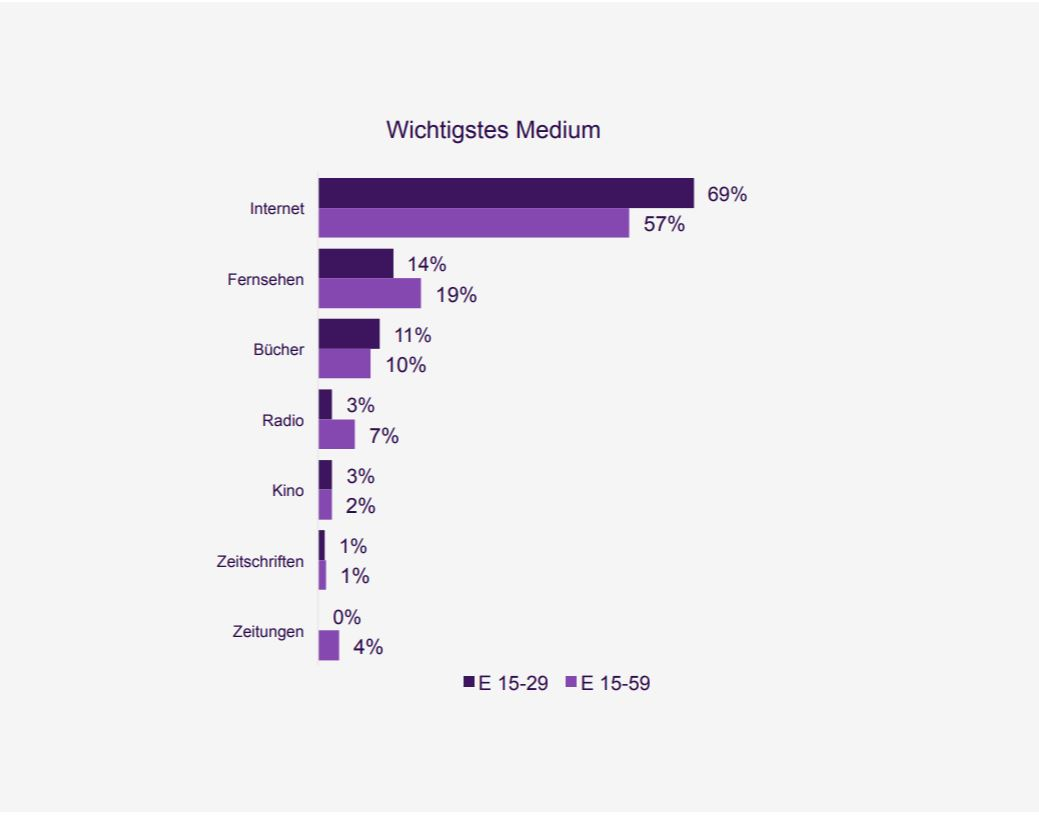
\includegraphics[width=14cm]{BilderAllgemein/Internetnutzung}\medskip
	\caption{Internetnutzung \cite{Geraetenutzung}}
	\label{fig:Internetnutzung}
\end{figure}

\begin{figure}[h]
	\centering
	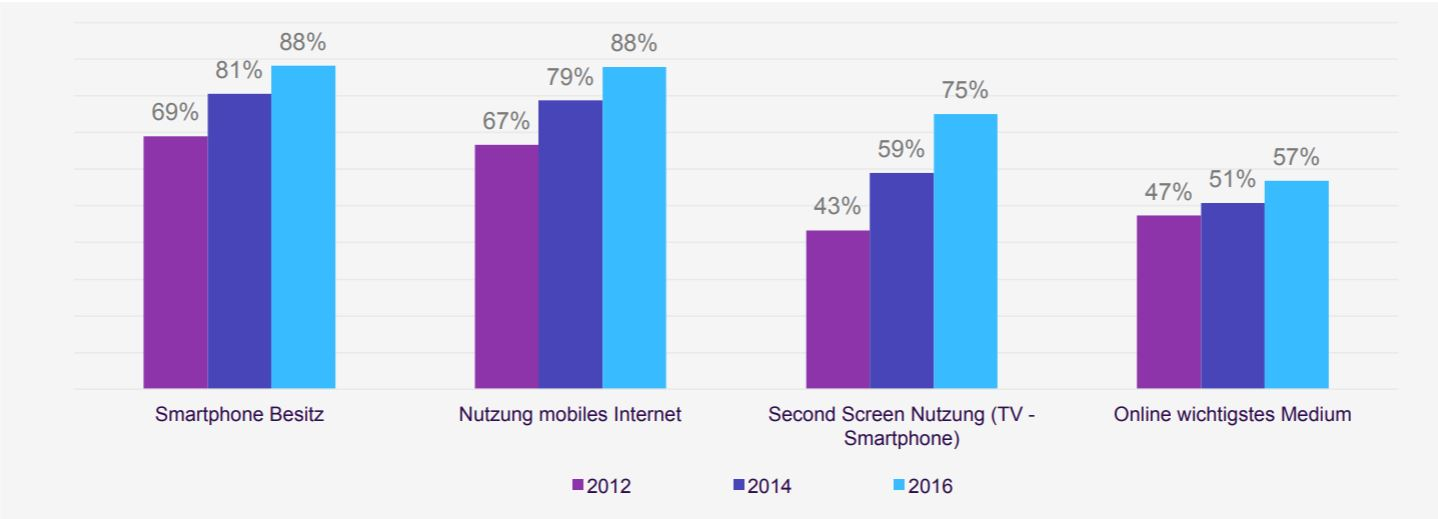
\includegraphics[width=14cm]{BilderAllgemein/SmartPhoneNutzung}\medskip
	\caption{Smartphonenutzung \cite{Geraetenutzung}}
	\label{fig:Smartphonenutzung}
\end{figure}







\section{Geschichte Softwareentwicklung}
Um die Geschichte der Softwareentwicklung darstellen zu können müssen wir als aller ersten die Frage stellen "Was ist Software?" und was wie ist eine Software definiert.
 
\subsection{Was ist Software}
Diese Frage stellen sich sicherlich alle mal die zum ersten Mal in ihrem Leben mit dieser Technologie in Berührung kommen. Eine genau Definition zu finden ist schwierig da die Software für die Gesamtheit eines Produktes steht . In \cite{WasistSoftware} ist die Softwaretechnik wie folgt definiert:

\begin{quote}

" Zielorientierte Bereitstellung und systematische Verwendung von Prinzipien, Methoden und Werkzeugen für
die arbeitsteilige, ingenieurmäßige Entwicklung und Anwendung
von umfangreichen Softwaresystemen. Zielorientiert bedeutet die
Berücksichtigung z.B. von Kosten, Zeit, Qualität." (\cite{WasistSoftware} Seite 17).
\end{quote}

Weiters wird in 

\begin{itemize}
    \item 
	\item 
	\item 
\end{itemize}



\newpage
\section{Desktop APP}


\section{Mobile APP}
Anfang des neues Jahrtausends war die Vorstellung, dass das Mobiltelefon  


\subsection{Native Apps}





\subsection{Webapplikationen}


\subsection{Progressive Web Apps}


\subsection{Unterschiede zwischen Web Apps PWA und Native Apps}

\newpage
